\documentclass{article}
\usepackage{../csci-246-fall2018/hw/template/fasy-hw}
\usepackage{amsmath}
\usepackage{cancel}
\usepackage{hyperref}

\author{Nathan Stouffer}
\problem{8-1}
% \problem{A-B} means Problem Set A, Problem B.
\collab{Kevin Browder}
% or give names, e.g., \collab{Alyssa P. Hacker and A. Student}

\begin{document}
	
Prove a tree always has one more vertex than edges. \\\\
Let $v$ be the number of vertexes in a given tree and $e$ be the number of edges in the same tree. Then, let the statement $A$ be $v=e+1$. We will prove $A$ via mathematical induction. \\\\
Base case: A tree with one edge and two vertices. In this case, $v=2$ and $e=1$. Then, the LHS of $A$ is $2$ and the RHS of $A$ is $1+1=2$. Therefore, LHS$=$RHS. \\\\
We will now assume $A$ is true for an arbitrary tree and prove $A$ to be true by adding an edge to an arbitrary tree. If there exists an arbitrary tree, there is only one way to increase the number of edges or vertices: by connecting an edge to a single, existing vertex. By doing this, $v$ is increased by one, and $e$ is also increased by one. This preserves the equivalence of $A$:
\begin{align*}
	(v+1)&=(e+1)+1 \\
	v+1&=e+2
\end{align*}
Thus, by mathematical induction, a tree always has one more vertex than edges.

\problem{8-2}
\collab{Kevin Browder}
\clearpage
\header

\begin{enumerate}[2.1]
	\item $T(n)=9T(\dfrac{n}{3})+n$ \\
		$a=9$, $b=3$, therefore, $c=\log_39=2$. If $f(n)=n=\mathcal{O}(n^{c-\epsilon}) =\mathcal{O}(n^{2-1}) =\mathcal{O}(n^1)$ for $\epsilon = 1>0$, then Case 1 of the Master's Theorem applies and $T(n)=\mathcal{\theta}(n^2)$. Let $g(n)=n$ be the function inside $\mathcal{O}(g(n))$. Notice, $f(n)=n=g(n)$ and since any function is $\mathcal{O}$ of itself $f(n)=\mathcal{O}(n)$ and $T(n)=\mathcal{\theta}(n^2)$.
	\item $T(n)=T(\dfrac{n}{2})+1$ \\
		$a=1$, $b=2$, therefore, $c=\log_12=0$. If $f(n)=1=\theta(n^0)=\theta(1)$. Since any function is $\theta$ of itself, Case 2 of Masters' Theorem applies and $T(n)=\theta(\log n)$
\end{enumerate}

\problem{8-3}
\collab{Kevin Browder}
\clearpage
\header

\begin{enumerate}[(a)]
	\item Decrypted message: "LET IT SNOW"
	\item To determine what the message was, I first thought the encryption method used a Cesar Cipher. However, after asserting that either O or R must correspond to a vowel and OR must correspond to a word, I decrypted the message using the keys that satisfied those conditions and found complete gibberish. I then looked at Piazza and discovered and Affine Cipher. I then iterated through different possible $a$ values coprime to 26 ($b$ being equal to $0$). This lead me to $a=5$. Thus the encryption formula is $(5*x + 0) \mod 26$.
\end{enumerate}

\problem{8-4}
\collab{Kevin Browder}
\clearpage
\header

\section*{Section 9.3, Problem 30}

Let $A=$ even that two people or more have the same birthday. To find $P(A)$, we will first find its complement, $P(A^c)$. $P(A^c)$ is the probability that, in a group of $n$ people, no one has the same birthday as any one else.
\begin{align*}
	P(A^c) &= \dfrac{365}{365} * \dfrac{364}{365} * \dfrac{363}{365} * \dfrac{362}{365} * \cdot \cdot \cdot \dfrac{365-(n+2)}{365} *\dfrac{365-(n+1)}{365} \\
	&= \dfrac{365-364-363-362- \cdot \cdot \cdot (365-(n+2)) - (365-(n+1))}{365^n} \\
	&= \dfrac{365!}{365^n * (365-n)!} \\
	&= \dfrac{n!*365!}{n! * 365^n * (365-n)!}	& \text{multiply by } \dfrac{n!}{n!} \\
	&= \dfrac{n! \binom{365}{n}}{365^n} & \text{by definition of binomial theorem}
\end{align*}
We will now find the smallest $n$ such that $P_n(A^c) \leq \dfrac{1}{2}$:
\begin{enumerate}
	\item $n=19$: $P_{19}(A^c) = \dfrac{19! \binom{365}{19}}{365^19} = 0.62$
	\item $n=24$: $P_{24}(A^c) = \dfrac{24! \binom{365}{24}}{365^24} = 0.46$
	\item $n=22$: $P_{22}(A^c) = \dfrac{22! \binom{365}{22}}{365^22} = 0.52$
	\item $n=23$: $P_{23}(A^c) = \dfrac{23! \binom{365}{23}}{365^23} = 0.49$
\end{enumerate}
$P_{23}(A) = 1 - P_{23}(A^c) = 1- .49 = .51$. Therefore, for the probability that two or more people have the same birthday to be greater than $\dfrac{1}{2}$, there must a group size $n=23$.

\problem{8-5}
\collab{Kevin Browder}
\clearpage
\header

The graph of example 1 with its dual is pictured in Figure 1. The dual is in pencil and the map is in black pen.
\graphicspath{ {dual} }
\begin{figure}[h]
	\centering
	\fbox{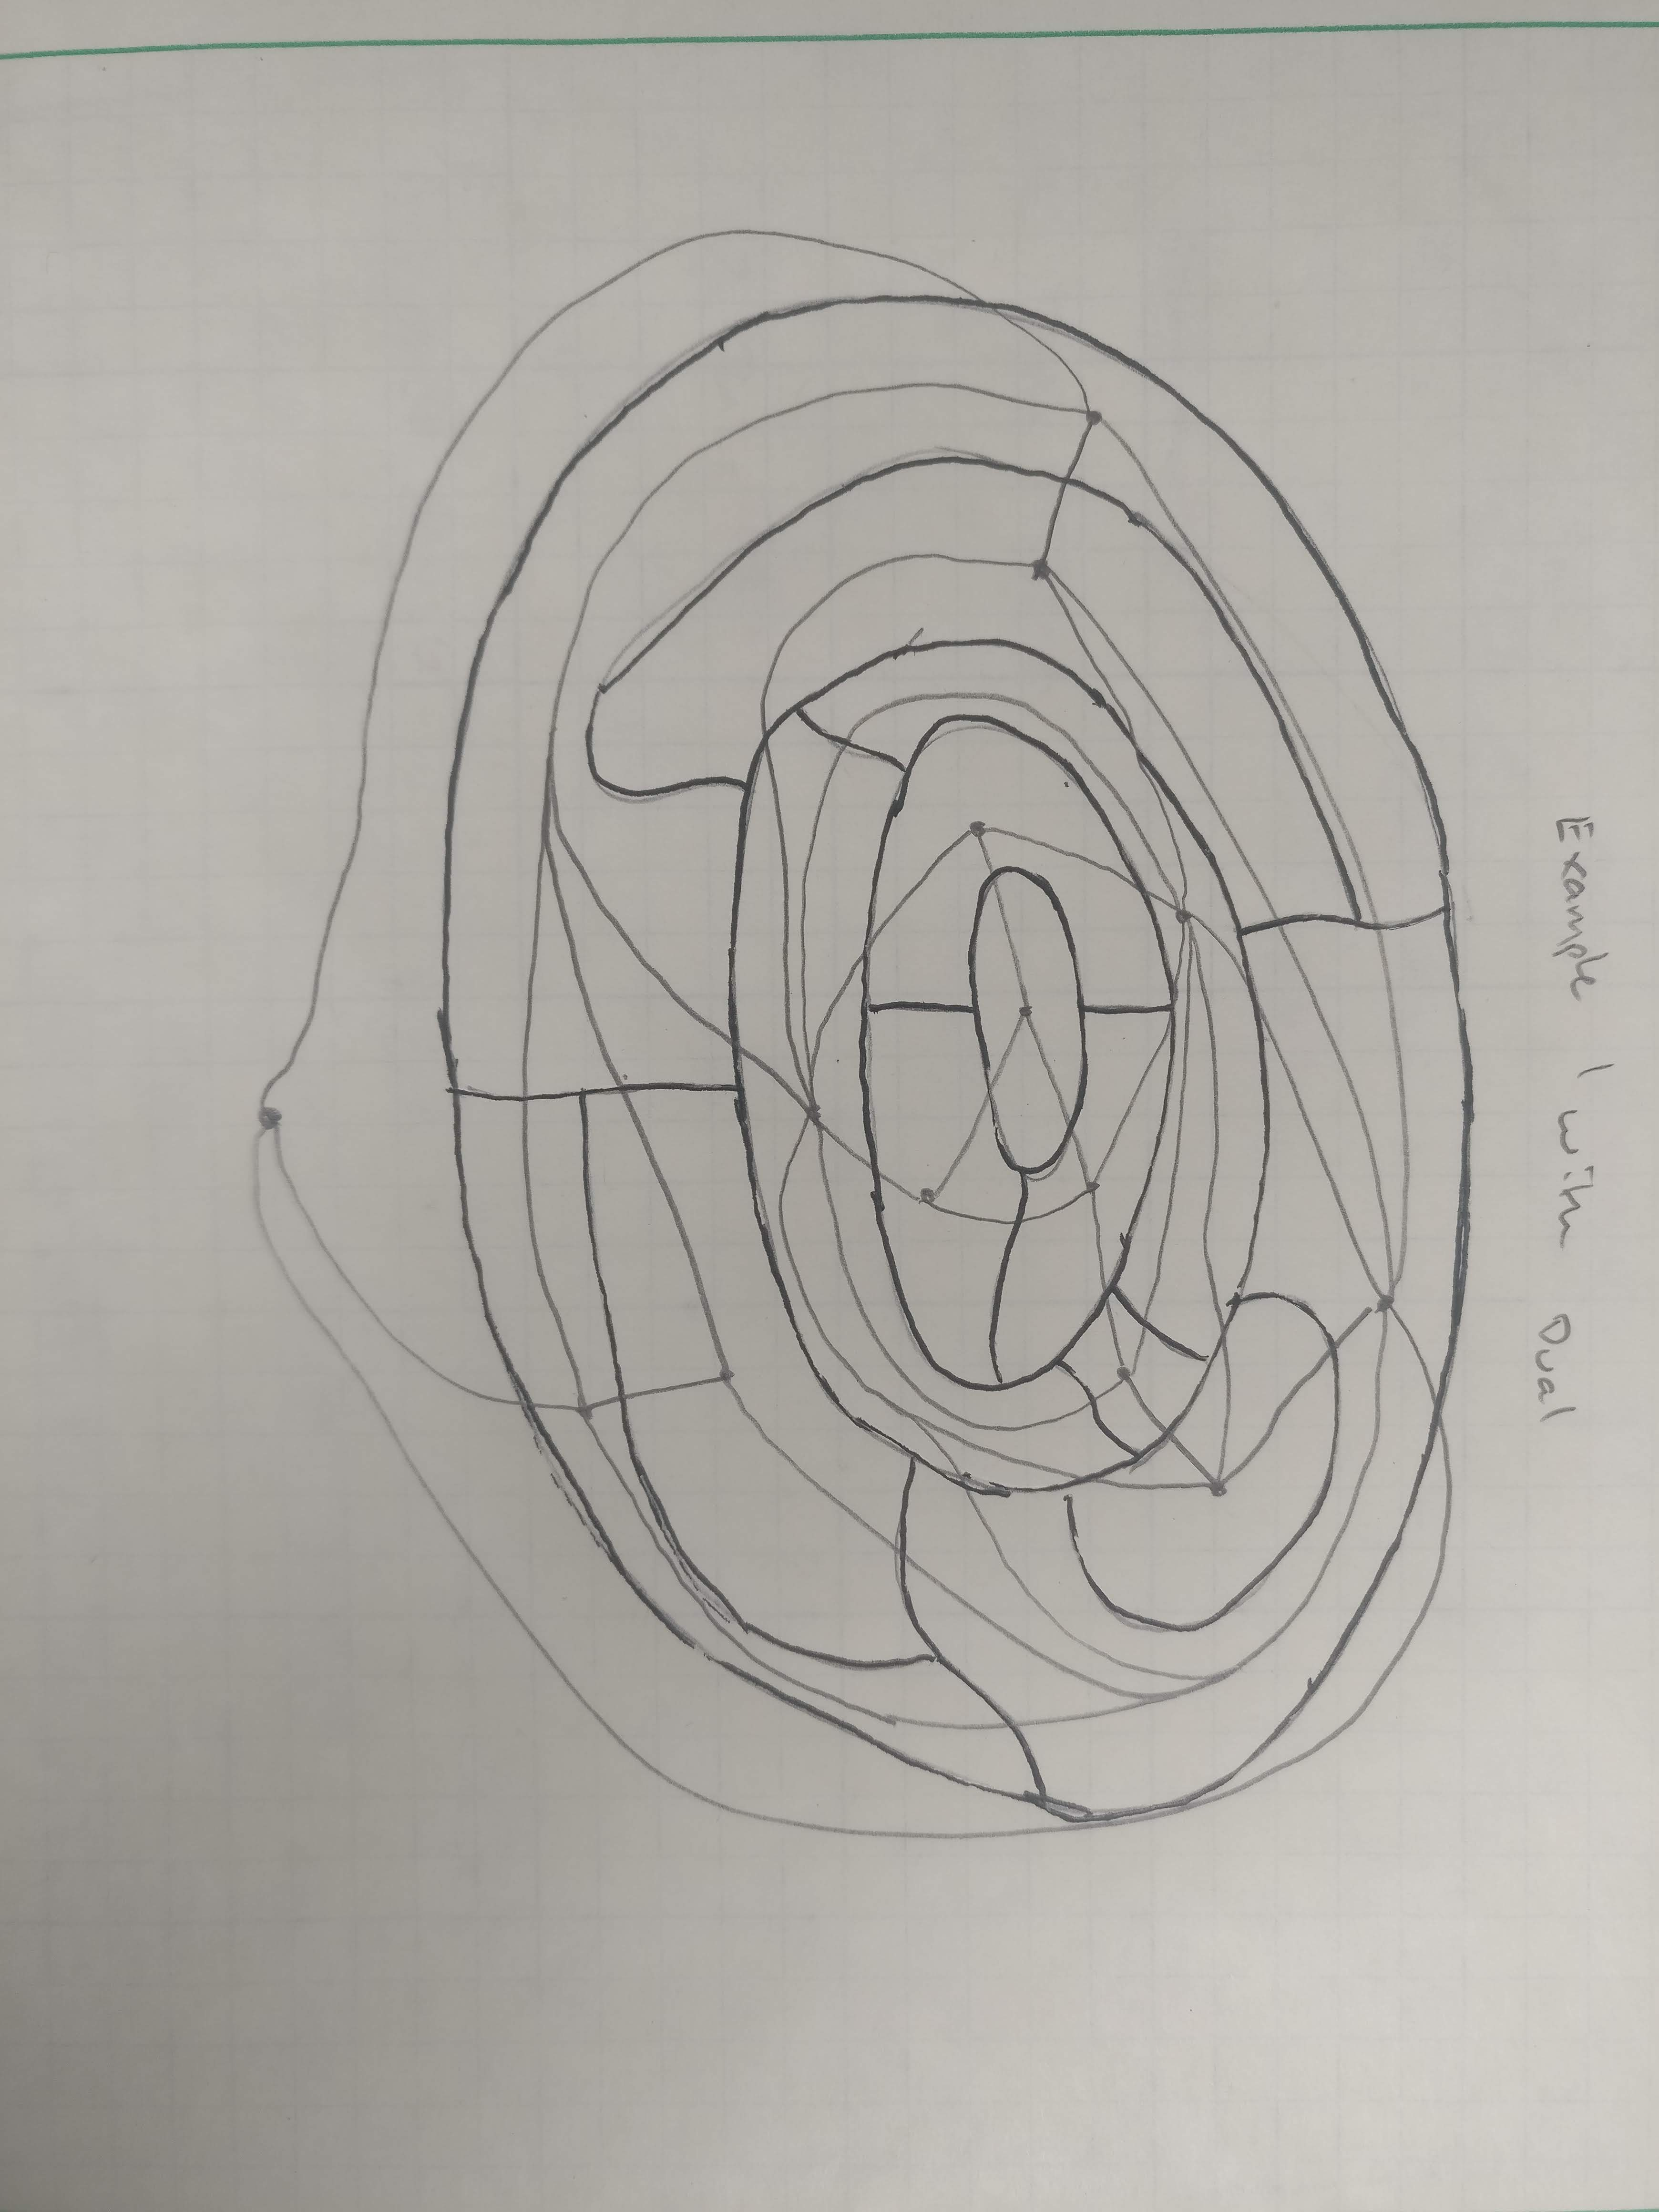
\includegraphics[angle=90, width=15cm]{dual}}
	\caption{Graph with Dual}
\end{figure}

\problem{8-6}
\collab{none}
\clearpage
\header

\section*{Grace Hopper}

References to online resources are provided as footnotes. \\

Grace Hopper is an American Computer Scientist born in the early 1900s who is one of the most famous women in computer science and developed the first compiler. According to the Encyclopedia Britannica, Hopper was "as a pioneer in developing computer technology."
\footnote{\url{https://www.britannica.com/biography/Grace-Hopper}}
The idea of Hopper's compiler is used constantly in computer science, even to compile this pdf. Without it, programmers would have to work far harder to code, which means it makes our lives easier.

\end{document}

